\documentclass[12pt]{article} \setlength{\oddsidemargin}{0in}
\setlength{\evensidemargin}{0in} \setlength{\textwidth}{6.5in}
\setlength{\parindent}{0in} \setlength{\textwidth}{16cm}
\setlength{\topmargin}{1in} \addtolength{\topmargin}{-1.5in}
\setlength{\textheight}{23cm} \setlength{\parskip}{0.75cm}

% Brackets
\usepackage{mathtools} \DeclarePairedDelimiter\ceil{\lceil}{\rceil}
\DeclarePairedDelimiter\floor{\lfloor}{\rfloor}

% Tikz settings
\usepackage{tikz} \usetikzlibrary{trees} \usetikzlibrary {positioning}
\definecolor {mypurple}{cmyk}{0.6,0.4,0.1,0} \definecolor
{myred}{cmyk}{0,0.3,0.3,0} \usetikzlibrary{fit,shapes.misc}

% Typesetting options
\usepackage{fancyvrb} \usepackage{amsmath,amsfonts,amssymb}
\usepackage [english]{babel} \usepackage [autostyle, english =
american]{csquotes} \usepackage[none]{hyphenat} \usepackage{url}

\begin{document}

\noindent CSCI 3104 Spring 2018 \hfill Problem Set 8\\
First Last (mm/dd)

% Image
\graphicspath{ {images/} }

\hrulefill

{\fontfamily{cmr}\selectfont}

% ******************* PROBLEM 1 *********************
\section*{Problem 1}

\textit{(10 pts) Ginerva Weasley is playing with the network given
  below. Help her calculate the number of paths from node 1 to node
  14.}

\textit{Hint: assume a ``path'' must have at least one edge in it to
  be well defined, and use dynamic programming to fill in a table that
  counts number of paths from each node j to 14, starting from 14 down
  to 1.}


\begin{figure}[h]
  \centering 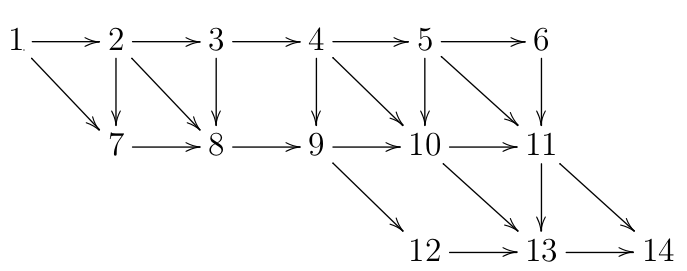
\includegraphics[width=0.8\textwidth]{P1}
\end{figure}

TODO

\newpage

% ******************* PROBLEM 2 *********************
\section*{Problem 2}

\textit{(10 pts) Ginny Weasley needs your help with her wizardly
  homework. She’s trying to come up with an example of a directed
  graph $G = (V, E)$, a start vertex $v \in V$ and a set of tree edges
  $E_T \subseteq E$ such that for each vertex $v \in V$, the unique path in the
  graph $(V, E_T)$ from $s$ to $v$ is a shortest path in $G$, yet the
  set of edges $E_T$ cannot be produced by running a depth-first
  search on $G$, no matter how the vertices are ordered in each
  adjacency list. Include an explanation of why your example satisfies
  the requirements.}
\\\\
TODO

\newpage

% ******************* PROBLEM 3 *********************
\section*{Problem 3}

\textit{(15 pts) Prof. Dumbledore needs your help to compute the in-
  and out-degrees of all vertices in a directed multigraph
  $G$. However, he is not sure how to represent the graph so that the
  calculation is most efficient. For each of the three possible
  representations, express your answers in asymptotic notation (the
  only notation Dumbledore understands), in terms of $V$ and $E$, and
  justify your claim.}

\begin{enumerate}
\item[(a)]{\textit{An \textbf{adjacency matrix} representation. Assume
      the size of the matrix is known.}}
  \\\\
  TODO
  \\
\item[(b)]{\textit{An \textbf{edge list} representation. Assume
      vertices have arbitrary labels.}}
  \\\\
  TODO
  \\
\item[(c)]{\textit{An \textbf{adjacency list} representation. Assume
      the vector’s length is known.}}
  \\\\
  TODO

\end{enumerate}

\newpage
% ******************* PROBLEM 4 *********************
\section*{Problem 4}

\textit{(30 pts) Deep in the heart of the Hogwarts School of
  Witchcraft and Wizardry, there lies a magical grey parrot that
  demands that any challenger efficiently convert directed multigraphs
  into directed simple graphs. If the wizard can correctly solve a
  series of arbitrary instances of this problem, the parrot will
  unlock a secret passageway.}

\textit{Let $G = (E, V)$ denote a directed multigraph. $A$ directed
  simple graph is a $G' = (V, E')$, such that $E'$ is derived from the
  edges in $E$ so that (i) every directed multiedge, e.g.,
  ${(u, v), (u, v)}$ or even simply ${(u, v)}$, has been replaced by a
  single directed edge ${(u, v)}$ and (ii) all self-loops $(u, u)$
  have been removed.}

\begin{figure}[h]
  \centering 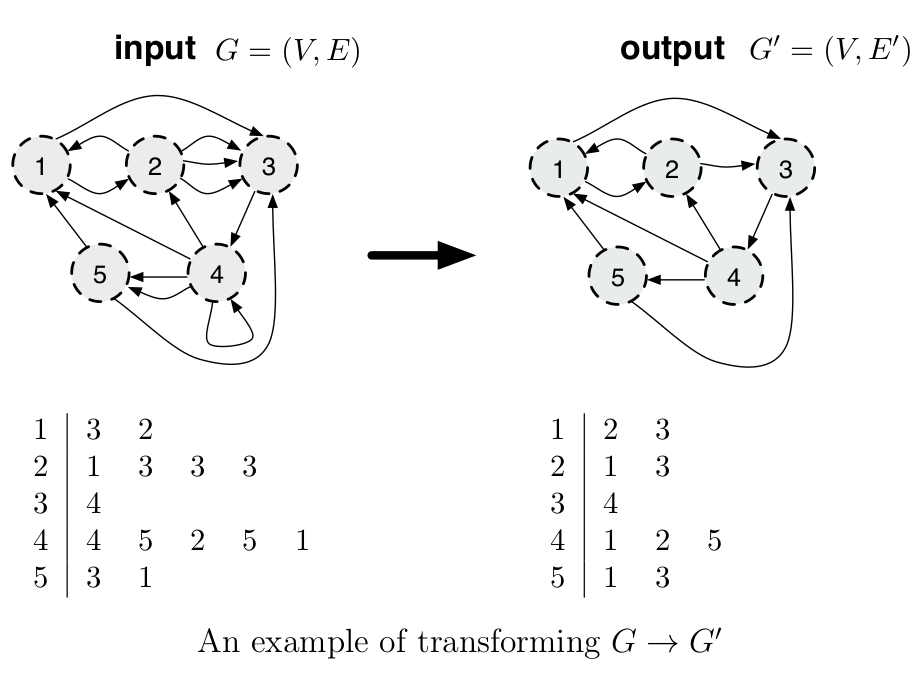
\includegraphics[width=1\textwidth]{P4}
\end{figure}

\textit{Describe and analyze an algorithm (explain how it works, give
  pseudocode if necessary, derive its running time and space usage,
  and prove its correctness) that takes $O(V + E)$ time and space to
  convert $G$ into $G'$, and thereby will solve any of the Sphinx’s
  questions. Assume both $G$ and $G'$ are stored as adjacency lists.}

\textit{Hermione’s hints: Don’t assume adjacencies \texttt{Adj[u]} are
  ordered in any particular way, and remember that you can add edges
  to the list and then remove ones you don't need.}
\\\\
TODO

\newpage


% ******************* PROBLEM 5 *********************
\section*{Problem 5}

\textit{(15 pts extra credit) Professor McGonagall has provided the
  young wizard Ron with three magical batteries whose sizes are 42,
  27, and 16 morts, respectively. (A mort is a unit of wizard energy.)
  The 27-mort and 16-mort batteries are fully charged (containing 27
  and 16 morts of energy, respectively), while the 42-mort battery is
  empty, with 0 morts. McGonagall says that Ron is only allowed to
  use, repeatedly, if necessary, the \textbf{mort transfer spell} when
  working with these batteries. This spell transfers all the morts in
  one battery to another battery, and it halts the transfer either
  when the source battery has no morts remaining or when the
  destination battery is fully charged (whichever comes first).}

\textit{McGonagall challenges Ron to determine whether there exists a
  sequence of mort-transfer spells that leaves exactly 12 morts either
  in the 27-mort or in the 16-mort battery.}

\begin{enumerate}
\item[(a)]{\textit{Ron knows this is actually a graph problem. Give a
      precise definition of how to model this problem as a graph, and
      state the specific question about this graph that must be
      answered.}}
  \\\\
  TODO
  \\
\item[(b)]{\textit{What algorithm should Ron apply to solve the graph
      problem?}}
  \\\\
  TODO
  \\
\item[(c)]{\textit{Apply that algorithm to McGonagall’s
      question. Report and justify your answer.}}
  \\\\
  TODO

\end{enumerate}
  
% ---------------------------------------------------
\end{document}
